\begin{figure}[h]
  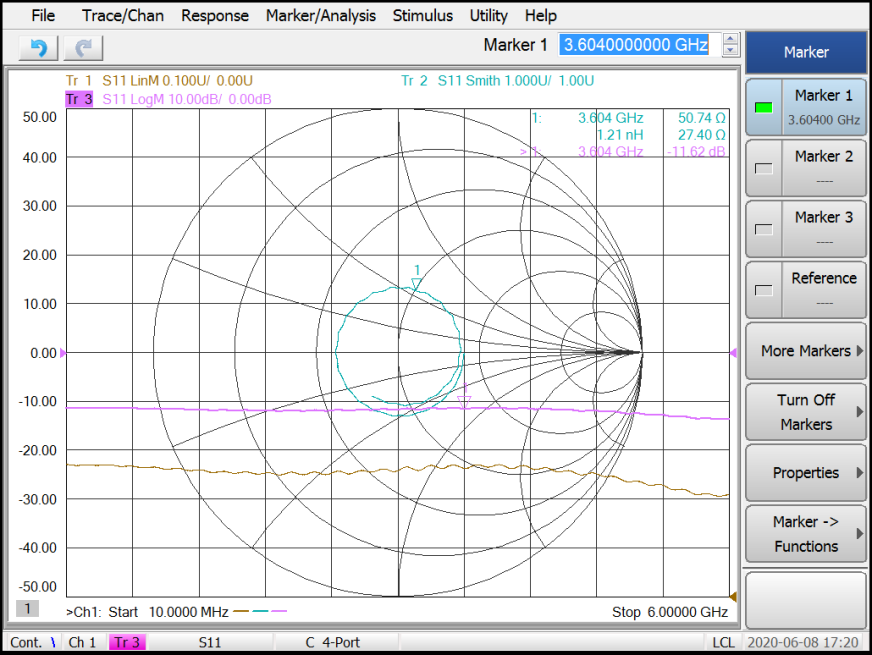
\includegraphics[width=\textwidth]{2_4}
  \caption{Smithdiagramm der S11-Messung des Dämpfungsgliedes}
  \label{fig:2_4_smith}
\end{figure}

Im Versuch wurde zuerst der S11-Parameter eines Dämpfungsgliedes bestimmt. Das
Ergebnis im Smith-Format ist in Abb. \ref{fig:2_4_smith} zu sehen.

Der Reflexionsfaktor zeigt eine Frequenzabhängigkeit, welche sich im
Smithdiagramm durch den kreisförmigen Verlauf (Abb. \ref{fig:2_4_smith} türkis)
äußert.

\begin{figure}[h]
  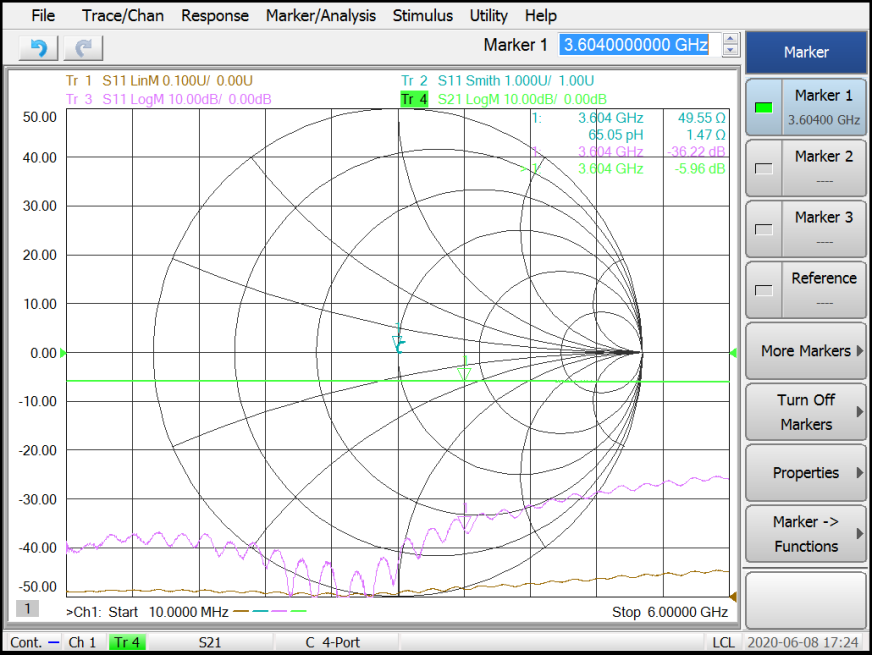
\includegraphics[width=\textwidth]{2_4_c_einfuge}
  \caption{Messung der Einfügedämpfung des Dämpfungsgliedes (grün)}
  \label{fig:2_4_einfuge}
\end{figure}

Mit einer Messung der Transmission/Einfügedämpfung und dafür notwendiger vorheriger Verbindung
eines zweiten Ports ergab sich die Übertragungsfunktion des Dämpfungsgliedes.
Die Einfügedämpfung ist in Abb. \ref{fig:2_4_einfuge} zu sehen. Man erkennt die konstante
Dämpfung von etwa $-5.96 \, \si{\deci\bel}$ über den betrachteten Frequenzbereich.

\begin{figure}[h]
  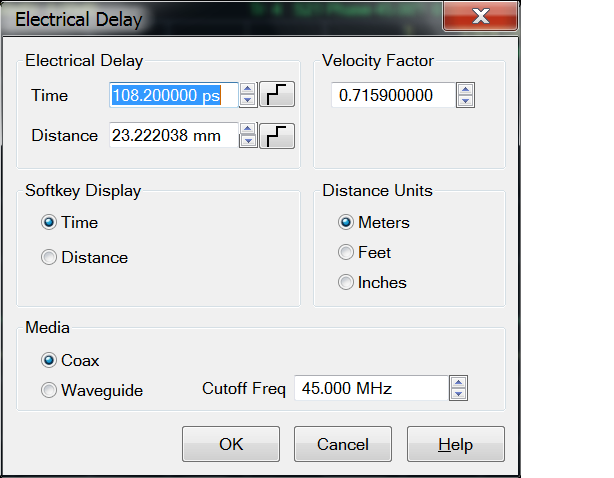
\includegraphics[width=\textwidth]{Elektrische_lange}
  \caption{Bestimmung der physikalischen Länge mithilfe des Electrical Delays}
  \label{fig:laenge1}
\end{figure}

Die ausschalggebende Größe für die Bestimmung der elektrischen bzw.
physikalischen Länge ist die Phase des Dämpfungsgliedes. Diese wurde gemessen
und das Electrical Delay angepasst, bis der Phasenverlauf inetwa $0
\si{\degree}$ im Frequenzgang entspricht. Über den voreingestellten
Verkürzungsfaktor im Fenster \emph{Electrical Delay} errechnete das Programm die
physikalische Länge des DUT (Abb. \ref{fig:laenge1}, \textit{Distance}), welche
mit der Messung durch ein Lineal positiv überprüft werden konnte.


